\begin{answer}
% Accuracy for college degree dataset: 90.0\% \\
% Accuracy for iris dataset: 93.33\% \\
\begin{figure}[H]
    \centering
    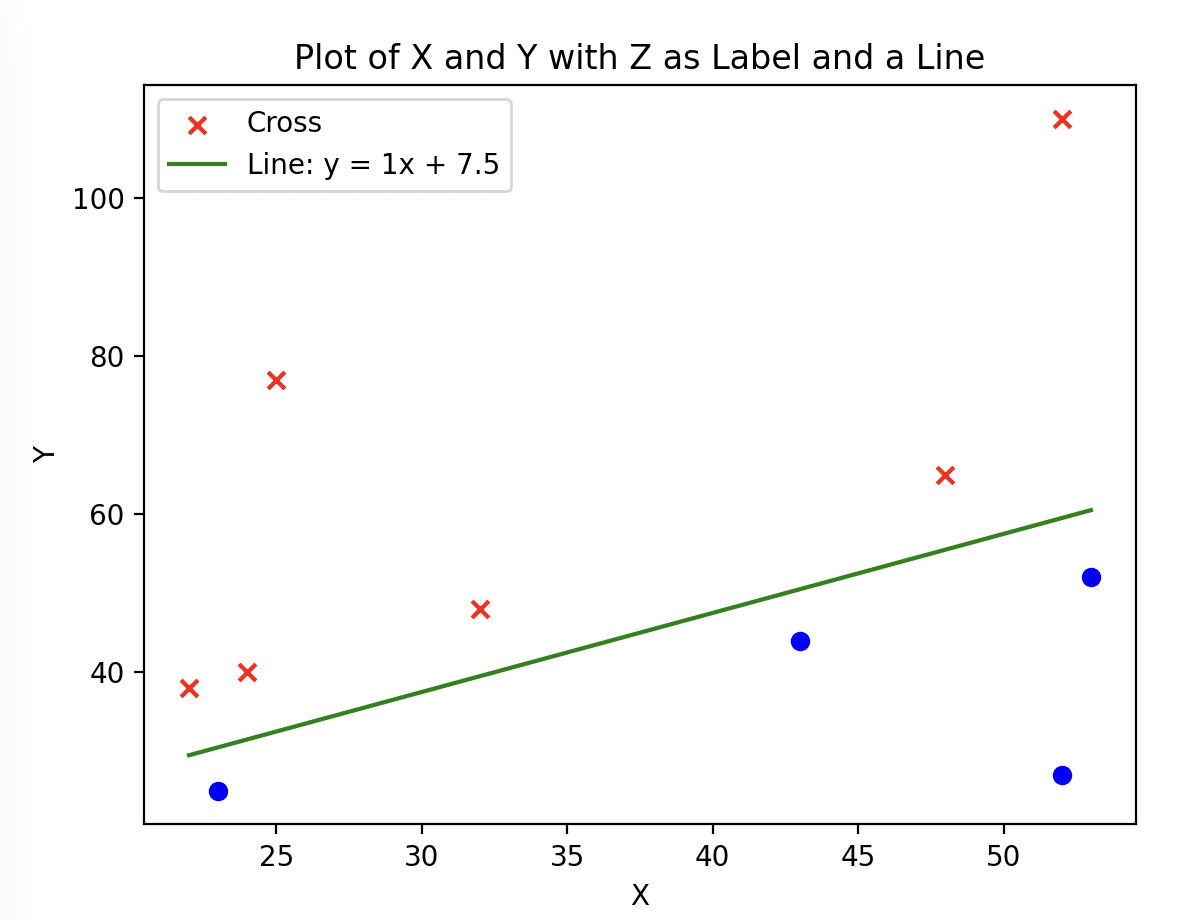
\includegraphics[width=0.5\linewidth]{Screenshot 2024-02-20 at 23.45.57.png}
    \caption{ps3::q1::c}
    \label{fig:enter-label}
\end{figure}

The above figure shows the training samples can be linearly separated by $income = age + 7.5$, this line is equivalent to 
\begin{equation}
    -0.13 \cdot  \text{age} + 0.13 \cdot  \text{income} - 1 = 0
\end{equation}

so $\alpha = -0.13$, $\beta = 0.13$. At root node the classification error is 4, and after one slipt, we get two leaf nodes with classification error = 0
\end{answer}